\documentclass[12pt]{article}
\usepackage{amsmath, amsthm, amssymb, amsfonts}
\usepackage{hyperref}
\usepackage{graphicx}

\DeclareMathOperator*{\argmin}{argmin}

%opening
\title{Flat Norm on Graphs}
\author{Sandy Auttelet, Jared Brannan, Blake Cecil, Curtis Michels,\\
 Katrina Sabochick, Kevin Vixie }

\begin{document}

\maketitle

\begin{abstract}
In this paper we implement and test a method for computing the multiscale flat norm signature for characteristic functions over irregular grids in $\mathbb{R}^2$ and $\mathbb{R}^3$.
\end{abstract}

\tableofcontents

\section{Multiscale Flat Norm}

In 2005, Chan and Esedoglu introduced an edge preserving total variation regularization functional:

\begin{equation} \label{ce}
F_{CE}(u) = \int_\Omega |\nabla u dx + \lambda \int_{\Omega} |u-f|dx
\end{equation}

Where $\Omega$ is a domain on which we have greyscale data $f:\Omega \to \mathbb{R}$ we would like to denoise. Solving the above we obtain:

\begin{align*}
u^* = \argmin_u F_{CE}(u)
\end{align*}

Which yields the denoised greyscale approximation $u^*:\Omega \to \mathbb{R}$ to the data $f$. The strength of the denoising may be adjusted by the parameter $\lambda \in [0,\infty)$, a large value of $\lambda$ corresponds to enacting a strict penalty for candidates $u$ that deviate too far from the original data and thus enforce less denoising. We henceforth refer to (\ref{ce}) as the $L^1$TV functional.

It was recognized in \cite{Morgan_2007} by Simon Morgan and Kevin Vixie that the $L^1$TV functional was both a special case of and an extension of the flat norm in geometric measure theory (GMT). Work was done in \cite{shapes} by Kevin Vixie Et al. to explore the implications of this.


\section{Discrete Implementations}

If $\chi_E$ is the characteristic function of $E$, with $\chi_E(x) = 1$ if $x \in E$ and $0$ otherwise, and $u$ may be taken to be of this form, then the $L^1$TV functional in (\ref{ce}) reduces to:

\begin{align*}
F_{CE}(\Sigma) &= \text{Per}(\Sigma) + \lambda|\Sigma \Delta \Omega|
\end{align*}

Where $\Sigma$ is the support of $u = \chi_\Sigma$, Per($\Sigma$) is the perimeter of $\Sigma$, and $\Sigma \Delta \Omega$ is the symmetric difference between $\Sigma$ and the support $\Omega$ of the data $f = \chi_\Omega$. 

The flat norm with scale $\lambda$ of an oriented $1$-dimensional set $T$ is given by:

\begin{equation} \label{fn}
\mathbb{F}(T) = \min_S \{V_1(T-\partial S) + \lambda V_2(S)\}
\end{equation}

Where $V_1$ is 1-dimensional volume (length), $V_2$ is 2-dimensional volume (area) and $S$ varies over $2$-dimensional regions. We refer to the pair of the 1D and 2D sets $\{T,S\}$ as the flat norm decomposition. By \cite{Morgan_2007} we have for fixed $\lambda$:

\begin{equation}
\mathbb{F}(\partial \Omega) = F_{CE}(\Sigma)
\end{equation}

with flat norm decomposition $\{\partial \Omega, \Sigma \Delta \Omega\}$, with $\partial \Omega$ denoting the measure theoretic boundary of $\Omega$. In \cite{shapes}, Kevin Et al. thus represented the problem of computing the flat norm as minimizing the $L^1$TV functional and computing the minimzer by graph cuts as introduced by \cite{kolmogorov}. Applied to images, this is realized by representing each pixel as a node on a rectangular grid which forms the working space. A characteristic function $\chi_\Omega$ is defined on the nodes which represents a black and white thresholded image. Graph edges are added between each node using 16 nearest neighbors in image space. Each of these edges are weighted by minimizing gradient computation error on known functions. After, a virtual sink ($t$) and a virtual source node ($s$) are added. The source node is connected to every node in $\Omega$ and the sink to every node on the grid not in $\Omega$. 

A particular cut of this graph corresponds has a capacity equal to the value of the flat norm $\mathbb{F}(S)$ for a set of nodes $S$ consisting of nodes $n$ for which either the edge $(n,s)$ or $(n,t)$ is in the cut. Any cut of the graph incurs a penalty proportional to the number of image nodes it cuts, with the penalty exactly equal to $V_1(T-\partial S)$ in (\ref{fn}) for parameter $\lambda$. Hence finding a cut with minimal capacity is the same as computing the flat norm. 

The vector of weights $w^*$ calculated in \cite{shapes} were chosen more specifically to approximate the function $g_\theta:\mathbb{R}^2 \to \mathbb{R}$ whose gradient is $\nabla g_\theta = (\cos \theta, \sin \theta)^T$ for all $\theta$:

\begin{equation}
w^* = \argmin_w \int_0^{2\pi} (h(w,\theta)-1)^2 d\theta
\end{equation}

With

\begin{align*}
h(w,\omega) &= \sum_{j=1}^4 w_1 |\nabla g_\theta \cdot v_j| + \sum_{j=5}^8 w_2 |\nabla g_\theta \cdot v_j| +  \sum_{j=9}^{16} w_4 |\nabla g_\theta \cdot v_j|
\end{align*}

Where $v_j, j= 1,...,16$ are the vectors from a fixed point in the grid to its 16 nearest neighbors, where three types of neighbor groupings are identified as below.

\begin{figure}
\centering
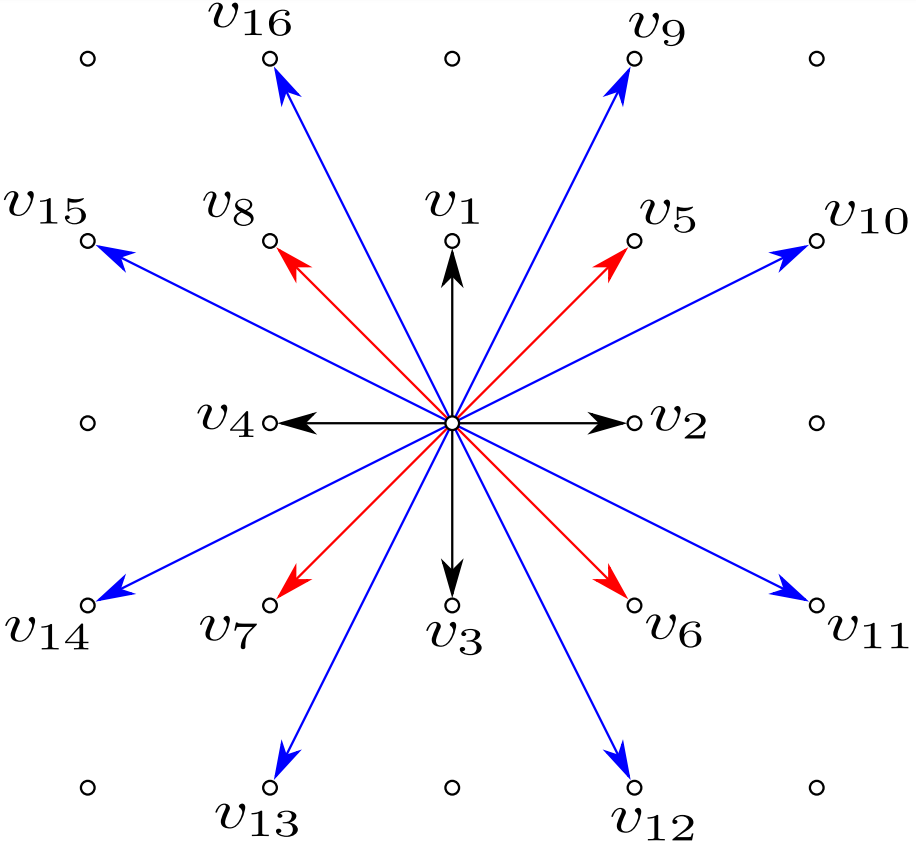
\includegraphics[scale=0.25]{Figure_2_Vixie_Paper.png}
\caption{16 vector neighborhood from \cite{shapes}.}
\end{figure}


\section{Flat Norm on Arbitrary 2D and 3D Graphs}

\section{Tests}

\section{Edge Cases}

\bibliographystyle{plain} % We choose the "plain" reference style
\bibliography{refs} % Entries are in the refs.bib file

\end{document}
